% ------------------------------------------------------------------------------
% TYPO3 CMS 6.2 LTS - What's New - Chapter "Responsive Images" (Italian Version)
%
% @author Roberto Torresani <roberto.torresani@typo3.org>
% @license	Creative Commons BY-NC-SA 3.0
% @link		http://typo3.org/download/release-notes/whats-new/
% @language	Italian
% ------------------------------------------------------------------------------
% Chapter: Responsive Images
% ------------------------------------------------------------------------------

\section{Immagini responsive}
\begin{frame}[fragile]
	\frametitle{Immagini responsive}

	\begin{center}\huge{Capitolo 2:}\end{center}
	\begin{center}\huge{\color{typo3darkgrey}\textbf{Immagini responsive}}\end{center}

\end{frame}

% ------------------------------------------------------------------------------
% Select Screen Size In Page Preview
% ------------------------------------------------------------------------------

\begin{frame}[fragile]
	\frametitle{Immagini responsive}
	\framesubtitle{Seleziona le dimensioni dello schermo nell'anteprima di pagina}

	\begin{itemize}
		\item Gli editor possono selezionare le dimensioni dello schermo nel modulo "View" per verificare i siti responsivi
	\end{itemize}

	\begin{figure}
		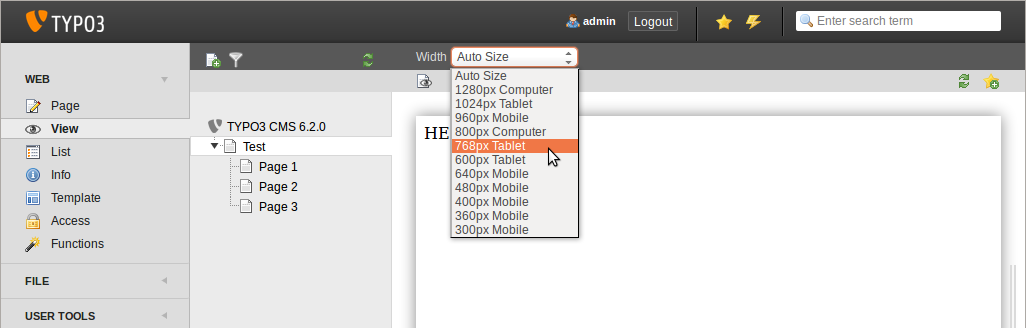
\includegraphics[width=0.95\linewidth]{Images/ResponsiveImages/ScreenSizeInPagePreview.png}
	\end{figure}

\end{frame}

% ------------------------------------------------------------------------------
% Customize Available Screen Sizes
% ------------------------------------------------------------------------------

\begin{frame}[fragile]
	\frametitle{Immagini responsive}
	\framesubtitle{Personalizzazione delle dimensioni di schermo}

	\begin{itemize}
		\item Le dimensioni dello schermo sono configurabili in PageTSconfig:

		\lstset{
			basicstyle=\fontsize{7}{9}\selectfont\ttfamily
		}

		\begin{lstlisting}
			mod.web_view.previewFrameWidths {
			  1780.label = <any LLL or string>
			  1780.height = 145
			}
		\end{lstlisting}

		\item La larghezza è definita dalla chiave (nell'esempio: 1780), l'altezza è un opzione
		\item Le dimensioni predefinite possono essere trovate nel file:\newline
			\small\texttt{typo3/sysext/core/Configuration/DefaultConfiguration.php}\normalsize
		\item Le etichette possono essere definite con PageTSconfig:

		\begin{lstlisting}
			mod.web_view.previewFrameWidths {
			  1280.label = LLL:EXT:viewpage/Resources/Private/Language/locallang.xlf:computer
			  1024.label = LLL:EXT:viewpage/Resources/Private/Language/locallang.xlf:tablet
			}
		\end{lstlisting}

	\end{itemize}

\end{frame}

% ------------------------------------------------------------------------------
% Responsive Image Galleries
% ------------------------------------------------------------------------------

\begin{frame}[fragile]
	\frametitle{Immagini responsive}
	\framesubtitle{Galleria delle immagini responsive}

	\begin{itemize}
		\item Attributi aggiuntivi per utilizzare gallerie di immagini responsive
		\item sono state aggiunte in "CSS styled content"
		\item Esempio: HTML5 (richiede \texttt{config.doctype = html5})\newline

			TYPO3 CMS < 6.2:

			\lstset{
				basicstyle=\fontsize{7}{9}\selectfont\ttfamily
			}

			\begin{lstlisting}
				<div class="csc-textpic-imagewrap">...</div>
			\end{lstlisting}

			TYPO3 CMS >= 6.2:

			\begin{lstlisting}
				<div class="csc-textpic-imagewrap"
				  data-csc-images="{register:imageCount}"
				  data-csc-cols="{field:imagecols}">...</div>
			\end{lstlisting}

	\end{itemize}

\end{frame}

% ------------------------------------------------------------------------------
% Responsive Image Rendering
% ------------------------------------------------------------------------------

\begin{frame}[fragile]
	\frametitle{Immagini responsive}
	\framesubtitle{Visualizzazione di immagine responsiva}

	\begin{itemize}
		\item La visualizzazione del cObject IMAGE usa una "sourceCollection" per supportare le varie dimensioni di schermo
		\item nel visualizzare immagini responsive per i cObjects "testo/immagine" e "immagini" richiedendo due configurazioni nel Constant Editor:

			\texttt{styles.content.imgtext.responsive}\newline
			\texttt{styles.content.imgtext.layoutKey}

		\item Le opzioni valide sono:

			\begin{itemize}
				\item \texttt{default}:	\tabto{2cm} default tag \texttt{<img>}
				\item \texttt{srcset}:	\tabto{2cm} \texttt{<img>}-tag con sorgente alternativa come attributo srcset
				\item \texttt{picture}:	\tabto{2cm} \texttt{<picture>}-tag con tag sorgente figlio
				\item \texttt{data}:	\tabto{2cm} \texttt{<img>}-tag con sorgente alternativa come attributo data
			\end{itemize}

	\end{itemize}

\end{frame}

% ------------------------------------------------------------------------------
% Property: layoutKey
% ------------------------------------------------------------------------------

\begin{frame}[fragile]
	\frametitle{Immagini responsive}
	\framesubtitle{Proprietà: layoutKey}

	\begin{itemize}
		\item \texttt{layoutKey} definisce il layout di visualizzazione\newline
			(è il codice HTML, utilizzato per il tag \texttt{<img>})
		\item Ogni opzione mostra un comportamento univoco per la visualizzazione dell'HTML
		\item L'opzione \texttt{default} visualizza il tag \texttt{<img>} tradizionalmente\newline
			(viene utilizzato se il sito non è responsivo)
		\item L'implementazione di un sito responsivo necessita di immagini con dimensioni differenti nelle varie risoluzioni e grandezza di schermo
		\item Dipende dal framework HTML, browser e libreria JavaScript (per il miglioramento progressivo):

			\begin{itemize}
				\item usa uno dei layout predefiniti o
				\item definisci un tuo layout personalizzato
			\end{itemize}

	\end{itemize}

\end{frame}

% ------------------------------------------------------------------------------
% Property: layout
% ------------------------------------------------------------------------------

\begin{frame}[fragile]
	\frametitle{Immagini responsive}
	\framesubtitle{Proprietà: layout}

			\lstset{
				basicstyle=\tiny\ttfamily
			}

			\begin{lstlisting}
				layoutKey = {$styles.content.imgtext.layoutKey}
				layout {
				  default {
				    element = <img src="###SRC###" width="###WIDTH###" height="###HEIGHT###" ###PARAMS###
				      ###ALTPARAMS### ###BORDER######SELFCLOSINGTAGSLASH###>
				  }
				  srcset {
				    element = <img src="###SRC###" srcset="###SOURCECOLLECTION###" ###PARAMS###
				      ###ALTPARAMS### ###SELFCLOSINGTAGSLASH###>
				    source = |*|###SRC### ###SRCSETCANDIDATE###,|*|###SRC### ###SRCSETCANDIDATE###
				  }
				  picture {
				    element = <picture>###SOURCECOLLECTION###<img src="###SRC###" ###PARAMS###
				      ###ALTPARAMS######SELFCLOSINGTAGSLASH###></picture>
				    source = <source src="###SRC###" media="###MEDIAQUERY###"###SELFCLOSINGTAGSLASH###>
				  }
				  data {
				    element = <img src="###SRC###" ###SOURCECOLLECTION### ###PARAMS###
				      ###ALTPARAMS######SELFCLOSINGTAGSLASH###>
				    source = data-###DATAKEY###="###SRC###"
				  }
				}
			\end{lstlisting}

\end{frame}

% ------------------------------------------------------------------------------
% Property: layout.[layoutKey].element
% ------------------------------------------------------------------------------

\begin{frame}[fragile]
	\frametitle{Immagini responsive}
	\framesubtitle{Proprietà: layout.[layoutKey].element}


	\begin{itemize}
			\item \lstinline!###SRC###!\newline
				URL per l'attributo: \texttt{src}

			\item \lstinline!###WIDTH###!\newline
				Larghezza dell'immagine (in pixel) per l'attributo: \texttt{width}

			\item \lstinline!###HEIGHT###!\newline
				Altezza dell'immagine (in pixel) per l'attributo: \texttt{height}

			\item \lstinline!###PARAMS###!\newline
				Parametri aggiuntivi come definiti nel cObject IMAGE

			\item \lstinline!###ALTPARAMS###!\newline
				Parametri alternativi aggiuntivi come definiti nel cObject IMAGE

	\end{itemize}

\end{frame}

% ------------------------------------------------------------------------------
% Property: layout.[layoutKey].element
% ------------------------------------------------------------------------------

\begin{frame}[fragile]
	\frametitle{Immagini responsive}
	\framesubtitle{Proprietà: layout.[layoutKey].element}

		\begin{itemize}
			\item \lstinline!###BORDER###!\newline
				Bordo (in pixel) per l'attributo: \texttt{border}

			\item \lstinline!###SELFCLOSINGTAGSLASH###!\newline
				Tag di chiusura, es. \texttt{<img ... />} invece di \texttt{<img ... >}\newline
				(dipende da \texttt{config.xhtmlDoctype} o \texttt{config.doctype})

			\item \lstinline!###SOURCECOLLECTION###!\newline
				Sorgente aggiuntiva dell'immagine, dipende dall'uso responsivo nel design.
				L'esatto valore è definito nella chiave: \texttt{layout.[layoutKey].source}

	\end{itemize}

\end{frame}

% ------------------------------------------------------------------------------
% Property: sourceCollection.[dataKey]
% ------------------------------------------------------------------------------

\begin{frame}[fragile]
	\frametitle{Immagini responsive}
	\framesubtitle{Proprietà: sourceCollection.[dataKey]}

	\begin{itemize}
		\item sourceCollection di default di EXT:css\_styled\_content
		\item è fortemente suggerito scrivere la propria sourceCollection

			\lstset{
				basicstyle=\tiny\ttfamily
			}

			\begin{lstlisting}
				sourceCollection {
				  small {
				    width = 200
				    srcsetCandidate = 600w
				    mediaQuery = (max-device-width: 600px)
				    dataKey = small
				  }
				  smallRetina {
				    if.directReturn = 1
				    width = 200
				    pixelDensity = 2
				    srcsetCandidate = 600w 2x
				    mediaQuery = (max-device-width: 600px) AND (min-resolution: 192dpi)
				    dataKey = smallRetina
				  }
				}
			\end{lstlisting}
	\end{itemize}

\end{frame}

% ------------------------------------------------------------------------------
% Further Resources (External Links)
% ------------------------------------------------------------------------------

\begin{frame}[fragile]
	\frametitle{Immagini responsive}
	\framesubtitle{Ulteriori risorse}

	\begin{itemize}
		\item Esempi di codice funzionante:\newline
			\small\url{http://wiki.typo3.org/Responsive_Image_Rendering}\normalsize

		\item Articolo di Sven Wolfermann su typo3.org:\newline
			\small\url{http://typo3.org/news/article/responsive-image-rendering-in-typo3-cms-62/}\normalsize

		\item W3C specification:\newline
			\small\url{http://www.w3.org/html/wg/drafts/srcset/w3c-srcset/}\newline
			\small\url{http://www.w3.org/TR/html-picture-element/}

		\item Lavori e progetti del "Responsive Image Community Group":\newline
			\small\url{http://responsiveimages.org}\normalsize

	\end{itemize}

\end{frame}

% ------------------------------------------------------------------------------

